\documentclass[11pt]{article}
\usepackage{natbib}
\usepackage{graphicx}

% Default margins are too wide all the way around. I reset them here
\setlength{\topmargin}{-.5in}
\setlength{\textheight}{9in}
\setlength{\oddsidemargin}{.125in}
\setlength{\textwidth}{6.25in}
\setlength{\topmargin}{-.5in}
\setlength{\textheight}{9in}
\setlength{\oddsidemargin}{.125in}
\setlength{\textwidth}{6.25in} 


\title{Filtering read alignments in BAM format} 
\author{Tonatiuh Pe\~{n}a-Centeno \\
University of Greifswald}
\date{\today}

 
\begin{document}  
\maketitle
\abstract{RNA-seq data has become an important source of information for tasks such as differential 
expression analysis and transcript quantification. Given that this new technology produces millions of 
such short-reads, bespoke methods and tools are required to process such big amounts of information. 
Furthermore, the introduction of the Sequence AlignMent Format (SAM) \citet{heng09:SAM} has meant that many of the state-of-the-art alignment tools (Bowtie, GMAP, etc.) now produce outputs in such format or in its binary version, aka BAM.

This note documents "filterBAM", a program designed to clean single and paired RNA-seq reads. The filter 
is based on filterPSL, a perl script written by Prof. Mario Stanke. Both filterPSL and filterBam are 
designed for the cleaning of data that will subsequently be applied to the gene prediction problem. 
Nevertheless, it should be possible to modify rather easily, if it is to be applied to a different type of 
application. filterBam is written in C++ and makes use of the Bamtools API \citet{barnett11:BamTools}.

\section{Main features}
filterBam is a C++ code that cleans alignment files in BAM format that is based on filterPSL, a Perl routine 
written by Prof. Mario Stanke for PSL files. filterBAM includes the following filtering options:

\begin{itemize}
	\item	Screens out unmapped alignments.
	\item	Screens out alignments that do not comply with a pre-defined coverage level (default=80\%).
	\item	Screens out alignments that do not comply with a pre-defined percentage of identity (default=92\%).
	\item	Screeens out alignments whose insert gaps do not comply with a pre-defined distance (default=10).
	\item	Filters in two modalities: single and paired-end reads, expecting paired-queries to be given the suffixes "/1", "/2" or ".f", ".r".
	\item	When in paired-read mode, it optionally writes to separate files a prospective list of common 
			target genes and of pairedness coverage.
	\item 	The filter should work fine for filtering data coming from 454 and Illumina but not for SOLiD technology.
\end{itemize}


\section{Single reads}
Depending on the sequencing technology, RNA-seq data might be produced as single or paired-end reads. In 
this section, operation of the filter is described in a step by step basis because the paired-read filter 
works almost in the same way. 



\begin{figure}
\begin{center}
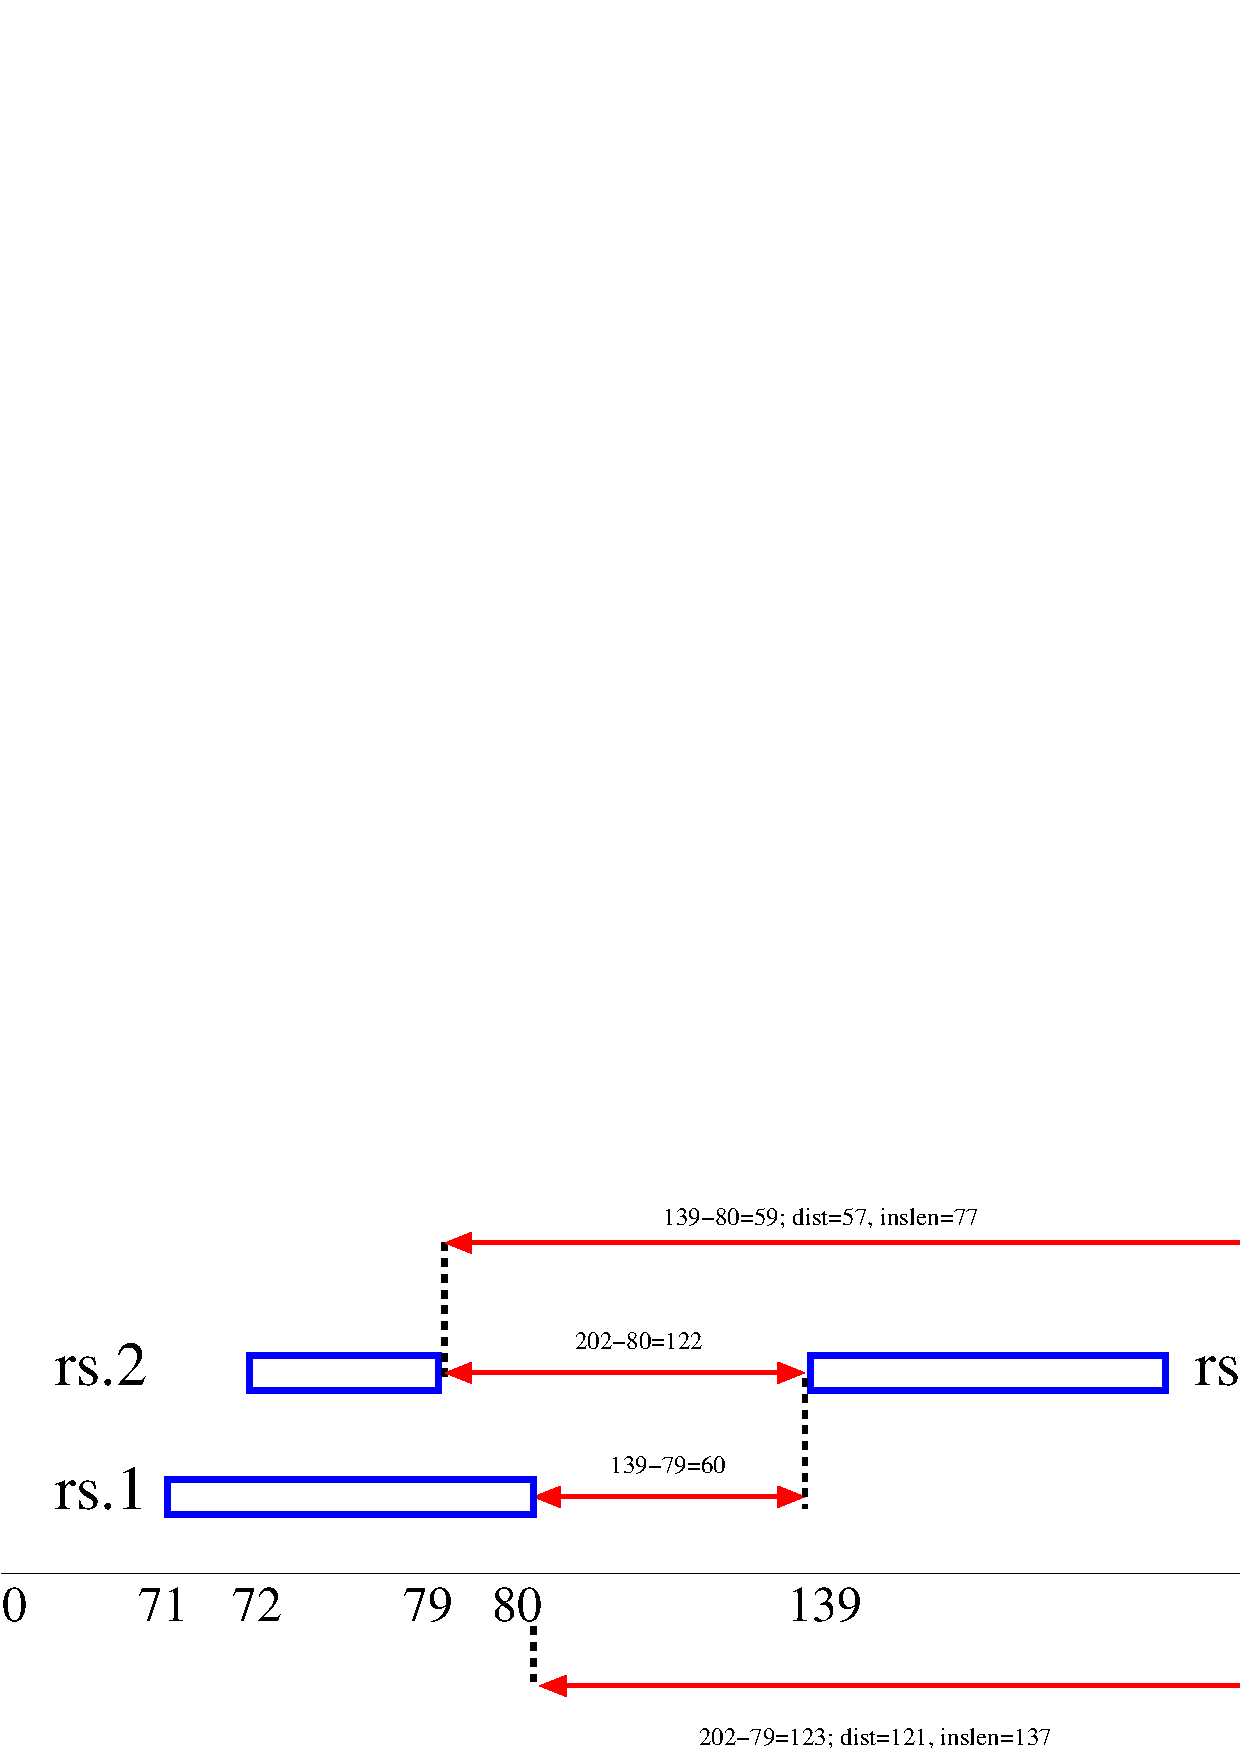
\includegraphics[width=7cm]{figures/pairedReads.pdf}
\end{center}
\end{figure}

\begin{figure}
\begin{center}
\includegraphics[width=7cm]{figures/similarFunction.pdf}
\end{center}
\end{figure}

\section{NOTES:}  
This document makes reference to the SAM/BAM format specification of \citet{heng09:SAM}.

\section{Bamtools}
Bamtools is a C++ wrapper API of the more well-known Samtools software. The latest version of Bamools 
is 2.0 and is available on the website 
	\begin{center}
		https://github.com/pezmaster31/bamtools/downloads
	\end{center}
\item 

\section{Test data}
We have generated a 

\section{Compilation}
Make sure to link with the ``-lz'' and ``-libbamtools.a'' flags on; where -lz refers to the ZLIB library, 
and libbamtools.a to the static bamtools library included in the software distribution. An example of 
how to compile and link follows: 

\begin{enumerate}
\begin{flushleft}
	\item	
		g++ -I\textbf{\$BAMTOOLS}/include   -g   -std=c++0x  -c filterBam.cc -o filterBam.o \\
	\item	g++     -g -std=c++0x  filterBam.o -o filterBam \textbf{\$BAMTOOLS}/lib/libbamtools.a -lz  
\end{flushleft}
\end{enumerate}
\vphantom{Nothing}
where \textbf{\$BAMTOOLS} is the path where Bamtools was installed.

Note that the flag ``-std=c++0'' has been used given that some of the functionalities of the filter require 
some of the newest features of GNU's g++ compiler. This and future versions of the software have been tested 
on Ubuntu's g++ version 4.4.3.

\section{How to run}
A run that will let pass most, if not all, readings: 
\begin{flushleft}
./filterBam input.bam output.bam --minCover 0 --minId 0  --insertLimit 10000000 --nointrons
\end{flushleft}
\textbf{Note:} that all options are provided at the very end.

\section{Coverage, percent of identity and insert length}
The coverage is computed as the sum of the alignment matches (sequence matches or mismatches) and 
the insertions to the reference. Both figures, alignment matches and insertions to the reference, correspond 
to CIGAR string operations $M$ and $I$, respectively. Thus the following is done 

\begin{equation}
	\mathrm{coverage} = \frac{\sum\mathrm{CIGAR}\left(M,I\right)}{qLength}
\end{equation}

An approximation to the percentage of identity is given by computing the query length and subtracting the 
so-called edit distance to the reference (tag ``NM'' in SAM jargon), i.e.

\begin{equation}
	\mathrm{percId} = \frac{qLength - \mathrm{Tag}(NM)}{qLength}
\end{equation}

The length of inserts is estimated by summing CIGAR operations ``M'' and ``I'', which correspond to alingment 
matches and deletions from the reference. In other words, we do the following

\begin{equation}
	\mathrm{InsertSize} = \frac{\sum\mathrm{CIGAR}\left(D,I\right)}{qLength}
\end{equation}


\begin{thebibliography}{1}
\providecommand{\natexlab}[1]{#1}
\providecommand{\url}[1]{\texttt{#1}}
\expandafter\ifx\csname urlstyle\endcsname\relax
  \providecommand{\doi}[1]{doi: #1}\else
  \providecommand{\doi}{doi: \begingroup \urlstyle{rm}\Url}\fi

\bibitem[Li et~al.(2009)Li, Handsaker, Wysoker, Fennell, Ruan, Homer, Math,
  Abecasis, Durbin, and Subgroup]{heng09:SAM}
H.~Li, B.~Handsaker, A.~Wysoker, T.~Fennell, J.~Ruan, N.~Homer, G.~Math,
  G.~Abecasis, R.~Durbin, and .~G. P. D.~P. Subgroup.
\newblock The sequence alignment/map format and samtools.
\newblock \emph{Bioinformatics Applications Note}, 25\penalty0 (16):\penalty0
  2078--2079, 2009.

\bibitem[Barnett et~al.(2011)Barnett, Garrison, Quinlan, Strömberg and Marth]{barnett11:BamTools}
D.~Barnett, E.~Garrison, A.~Quinlan, M.~Strömberg, G.~Marth.
\newblock BamTools: a C++ API and toolkit for analyzing and managing BAM files.
\newblock \emph{Bioinformatics}, 27\penalty0 (12):\penalty0
  1691-1692, 2011.


\end{thebibliography}


%\bibliographystyle{abbrvnat}

\end{document}
